%!TEX root = ../CallenThermo.tex
%----------------------------------------------------------------------------------------
%	翻译:哪吒儿闹海
%   校对:lh1962
%----------------------------------------------------------------------------------------


\chapter{热力学系统的稳定性}
\label{chap8}
\section{热力学系统的内在稳定性}
\label{sec8.1}
热力学中基本的极值原理指出:$\text{d}S=0$以及$\text{d}^2S<0$。第一个式子表示系统的熵取极值,第二个表明这个极值是极大值. 第二个式子决定着系统的{\it 稳定性},然而之前我们还没有完整地考察过这个式子. 与此相似,在力学中,一个单摆的稳定位置是其势能最小的位置. 而所谓处在“不稳定平衡”的位置与此相反,它正好在势能最大的地方.

对稳定性的考量将催生一些热力学中有趣且重要的结论. 在本章中考察可使系统达到稳定的条件. 在第9章中我们会讨论不稳定性的结果——相变.

现在考虑两个完全相同的子系统,它们的基本方程都是$S=S(U,V,N)$,这两个子系统由完全不透的隔板分开. 假设$S$对$U$的依赖关系大致如图\ref{fig8.1}所示. 现在我们从第一个子系统中挪出$\Delta U$的能量到第二个系统中去,这时,总系统(由这两个子系统所组成)的熵就会由$2S(U,V,N)$变为$S(U+\Delta U,V,N)+S(U-\Delta U,V,N)$. 由图中可看出,总系统的熵竟然增大了\mpar{请回忆 Jensen 不等式,并批判性的看待作者的讨论。}. 显然,如果绝热限制被移除,那么能量就会自发地从一子系统流向另一个子系统,因之其中一个的能量会增多(温度也增加),另一个的能量减少. 这种情况甚至可以发生在一个子系统内,即能量从一个区域自发地转移到另一个区域,导致系统的均一性被破坏. 这种均一性的自发破缺就是相变的特征.

\begin{figure}
\centering
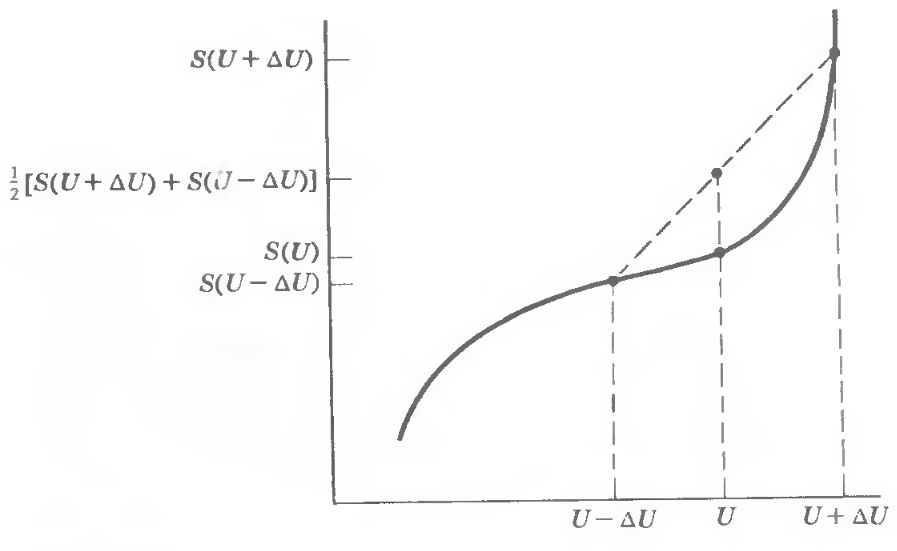
\includegraphics[width=\textwidth]{Pictures/fig8.1.png}
\figcaption{如图所示,对于下凹的基本关系,通过两个子系统的能量交换,平均熵增加了,这样的系统是不稳定的。}
\label{fig8.1}
\end{figure}

从图\ref{fig8.1}中我们可以看出,系统稳定的条件就是熵曲线{\it 上凹}.\footnote{R. B. Griffiths, \textit{J. Math. Phys.} \textbf{5}, 1215 (1964). L. Galgani and A. Scotti, \textit{Physica} \textbf{40}, (1968);\textbf{42},242(1969); \textit{Pure and Appl Chem.} \textbf{22}, 229(1970).}

\begin{equation}
\label{equ8.1}
S(U+\Delta U,V,N)+S(U-\Delta U,V,N)\leq 2S(U,V,N) \quad(\text{for all }\Delta)
\end{equation}

如果$\Delta U\to 0$,那么该条件就变为微分式
\begin{equation}
\label{equ8.2}
\left(\frac{\partial^2S}{\partial U^2}\right)_{V,N}\leq 0
\end{equation}
但是这个微分式没上凹条件\eqref{equ8.1}那么严格
,上凹条件需对所有的$\Delta U$成立,而非仅仅在$\Delta\to 0$时成立.

上面我们考虑的是能量的变化,如果我们考察体积的变化,结果是一样的
\begin{equation}
\label{equ8.3}
S(U,V+\Delta V,N)+S(U,V-\Delta V,N)\leq 2S(U,V,N)
\end{equation}
或写成微分形式
\begin{equation}
\label{equ8.4}
\left(\frac{\partial^2S}{\partial V^2}\right)_{U,N}\leq 0
\end{equation}

\begin{figure}
\centering
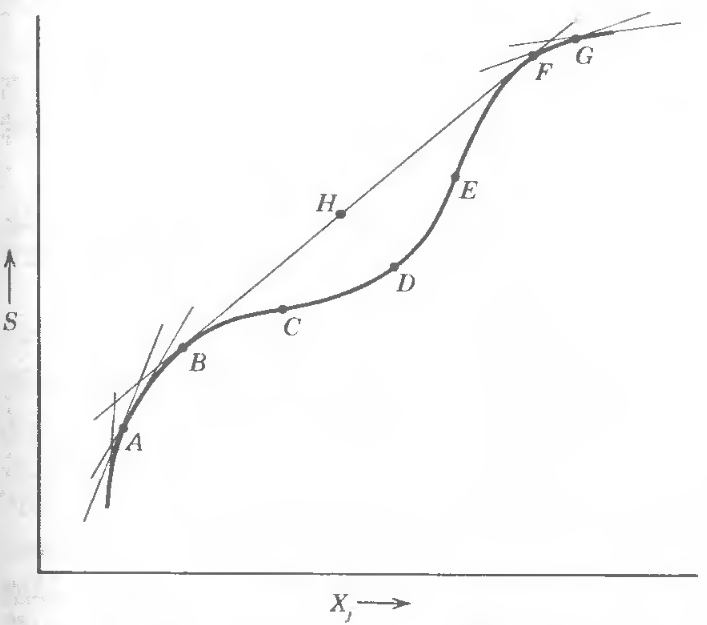
\includegraphics[width=.8\textwidth]{Pictures/fig8.2.png}
\figcaption{}
\label{fig8.2}
\end{figure}

在由统计力学计算所得和实验数据外推所得的基本方程中,有一些确实不满足上凹条件.这时如果非要得到一个稳定的基本方程的话,我们可以按照图\ref{fig8.2}所示的方法构造. 在真实的基本方程曲线上作切线,取那些处在曲线上方的切线,{\it 稳定的状态方程就是这些取出来的切线的上包络线}.

图\ref{fig8.2}中,BCDEF线是不稳定的,这一可用直线BHF来代替. 实际上,真实的状态方程中,只有CDE段不满足微分形式的稳定性条件(也就是说局部不满足上凹条件). 因此整个曲线就不满足“全局”性的上凹条件\eqref{equ8.1}.所以我们说该曲线中的BC和EF部分都是局域稳定但全局不稳定的.

直线(图\ref{fig8.2}中的BHF)对应着两个相的分离,即系统中的一部分处于B状态,而另一部分处于F状态,我们将在第9章中详细解释这个问题.

在$S-U-V$组成的三维空间中,全局稳定要求熵曲面处于它的所有切面之下. 也就是说
\begin{equation}
\label{equ8.5}
S(U+\Delta U,V+\Delta V,N)+S(U-\Delta U,V-\Delta V,N)\leq 2S(U,V,N)
\end{equation}
由该式可推得\eqref{equ8.2}、\eqref{equ8.4}和(参见问题8.1-1)
\begin{equation}
\label{equ8.6}
\frac{\partial^2S}{\partial U^2}\frac{\partial^2S}{\partial V^2}-\left(\frac{\partial^2S}{\partial U\partial V}\right) \ge 0
\end{equation}
我们待会儿会通过另一种方法得到这个等式:将一个类似\eqref{equ8.2}式的简单的曲率条件代入熵的Legendre变换.

再次强调,全局稳定要求熵曲面处于它的所有切面之下. 相较之下,局部稳定要求的条件就弱一些,它只要求$\left(\frac{\partial^2S}{\partial U^2}\right)_{V,N}$和$\left(\frac{\partial^2S}{\partial V^2}\right)_{U,N}$都是负的且$\frac{\partial^2S}{\partial U^2}\frac{\partial^2S}{\partial V^2}-\left(\frac{\partial^2S}{\partial U\partial V}\right)^2$是正的.
$\frac{\partial^2S}{\partial U^2}<0$保证了:体积为常数的平面与S-U-V曲面的交线曲率为负(线上每一处都是平衡点).同样,$\frac{\partial^2S}{\partial V^2}<0$保证了:能量为常数的平面与S-U-V曲面形成的交线曲率为负.
这两个“偏曲率(partial curvatures)”并不能保证曲面上凹,因为曲面上可能这样一种凹槽,它在$\pm U, \pm V$四个方向上曲率为负,但在四个对角方向($U,V$坐标轴之间的对角线)上曲率为正. 第三个微分关系\eqref{equ8.6}正是限制了这种情况的发生.

以物理的语言来说,局域稳定条件保证了系统中各部分的$u$或$v$各自的涨落不会导致熵增加,也保证了$u$、$v$共同的涨落不会导致熵增加.

对于磁体系而言也有类似的关系,只不过磁矩代替了体积的角色\footnote{R. B Griffiths, {\it J. Math. Phys.} {\bf 5}, 1215 (1964)} .

在彻底阐明这些稳定条件之前,我们先来考察一下其他类似的关系(不同的热力学势有不同的关系).我们先看一个意义最明显的关系\eqref{equ8.3}式,搞清楚它蕴含的信息,其他的关系也包含着类似的东西. 方程\eqref{equ8.2}要求
\begin{equation}
\label{equ8.7}
\left(\frac{\partial^2S}{\partial U^2}\right)_{V,N}=-\frac{1}{T^2}\left(\frac{\partial T}{\partial U}\right)_{V,N}=-\frac{1}{NT^2c_v}\leq 0
\end{equation} 
{\it 因此,一个稳定系统的摩尔热容必须为正.} 类似地。其他稳定性条件也会对一些可观测物理量作出限制.

最后我们做个总结,在一个$r+2$维的热力学空间$(S,X_0,X_1,\cdots,X_r)$中,{\it 系统的稳定性要求熵曲面处于它的所有切平面之下.}



\section{其他热力学势的稳定性条件}\label{sec8.2}
在能量表象下重新表述稳定性准则,只需要在语言上简单作一个转换就行. 既然要求熵最大能量最小,那么熵曲面的上凹性就可以转化为能量曲面的{\it 下凹性}.

稳定的能量曲面总处于它的切平面之上.
\begin{equation}
\label{equ8.8}
U(S+\Delta S,V+\Delta V,N)+U(S-\Delta S,V-\Delta V,N)\geq 2U(S,V,N)
\end{equation}

局域下凹条件变为
\begin{equation}
\label{equ8.9}
\frac{\partial^2U}{\partial S^2}=\frac{\partial T}{\partial S}\geq 0\qquad \frac{\partial^2U}{\partial V^2}=-\frac{\partial P}{\partial V}\geq 0
\end{equation}

附加$S,V$一同变化时的限制条件
\begin{equation}
\label{equ8.10}
\frac{\partial^2U}{\partial S^2}\frac{\partial^2U}{\partial V^2}-\left(\frac{\partial^2U}{\partial S\partial V}\right)^2\geq 0
\end{equation}

更严格一些的做法是:对能量或熵进行Legendre变换. 首先复习一些勒让德变换得性质(见式\eqref{equ5.31})
\begin{equation}
\label{equ8.11}
P=-\frac{\partial U}{\partial X}\qquad\text{及}\qquad X=-\frac{\partial U[P]}{\partial P}
\end{equation}

因之

\begin{equation}
\label{equ8.12}
\frac{\partial X}{\partial P}=-\frac{\partial^2U[P]}{\partial P^2}=\dfrac{1}{\frac{\partial^2U}{\partial X^2}}
\end{equation}

所以$\partial^2U[P]/\partial P^2$与$\partial^2U/\partial X^2$的符号相反.那么,{\it 如果$U$是$X$的一个上凹函数,则$U[P]$是一个关于$P$的下凹函数.} 用同样得方式可知,Helmholtz势是温度的上凹函数,是体积的下凹函数.
\begin{equation}
\label{equ8.13}
\left(\frac{\partial^2 F}{\partial T^2}\right)_{V,N}\leq 0\qquad \left(\frac{\partial^2 F}{\partial V^2}\right)_{T,N}\geq 0
\end{equation}

焓是熵的上凹函数,压强的下凹函数
\begin{equation}
\label{equ8.14}
\left(\frac{\partial^2 H}{\partial S^2}\right)_{P,N}\geq 0\qquad \left(\frac{\partial^2 H}{\partial P^2}\right)_{S,N}\leq 0
\end{equation}
Gibbs 势同时是温度和压强的下凹函数
\begin{equation}
\label{equ8.15}
\left(\frac{\partial^2 G}{\partial T^2}\right)_{P,N}\leq 0\qquad \left(\frac{\partial^2 G}{\partial P^2}\right)_{T,N}\leq 0
\end{equation}

总结起来,$N$恒定时,{\it 对各个热力学势的特征变量而言,对应热力学势($U$及其Legendre变换)是强度量的下凹函数,广延量的上凹函数. 同样地,$N$恒定时Massieu函数(熵及其Legendre变换)是对应强度量的上凹函数,广延量的下凹函数.}

\section{热力学系统的内在稳定性}
\label{sec8.3}
由稳定性准则能导出哪些物理结论?本节将讨论这个问题.稳定性准则将限制诸如$c_v, c_p,\alpha,\kappa_T$这些量的正负.第一个推论为:$c_v>0$,可由\eqref{equ8.2}或\eqref{equ8.7}式导出. 类似地,由Helmholtz势关于体积$V$的上凹性将得到
\begin{equation}
\label{equ8.16}
\left(\frac{\partial^2F}{\partial V^2}\right)_T=-\left(\frac{\partial P}{\partial V}\right)_T=\frac{1}{V_{\kappa_T}}\ge 0
\end{equation}
或
\begin{equation}
\label{equ8.17}
\kappa_T\ge 0
\end{equation}

由$c_v, \kappa_T$为正还能获得更多的信息。如果回想一下在问题3.9-5中所得的等式
\begin{equation}
\label{equ8.18}
c_p-c_v=\frac{Tv\alpha^2}{\kappa_T}
\end{equation}
和
\begin{equation}
\frac{\kappa_s}{\kappa_T}=\frac{c_v}{c_P}
\end{equation}
结合之前稳定性准则导出的结论,我们马上就能知道
\begin{equation}
c_p\ge c_v\ge 0
\end{equation}
和
\begin{equation}
\kappa_T\ge\kappa_s\ge 0
\end{equation}

因此在一个稳定系统中,热容和压缩率一定是正的. 即:\textsl{向满足稳定性准则的系统中加入热量,无论于恒压或恒容条件下,都将增加系统的温度——且恒容时比恒压时增加得更多.减少系统的体积,无论于绝热或恒温条件下,都将增大系统的压强——且绝热时比恒温时增加得更多}

\section{Le Chatelier 原理;涨落的定性影响}
\label{sec8.4}
稳定性准则的物理内涵就是著名的Le Chatelier 原理. 据该原理,稳定性可描述为:\textsl{系统中发生的会产生不均一性的事件的都会诱发一个趋向于抵消该事件的过程.}

举个例子,考虑一容器中处于平衡的液体,某时刻一光子射入液体,它将液体局部稍稍加热了一点. 根据稳定性条件,热量会从被加热的区域流走,被加热区域的温度因此而向周围环境的温度靠近,系统重建了平衡.

与此相类,液体中传播的纵波会让系统中一些地方的密度或高或低. 如果某区域密度增高,那么压强也随之增高,因而该处的液体趋向于散开,反之密度低的区域将趋向于收缩.稳定性条件(即压缩率为正)确保了这些响应将使系统重建平衡.

实际上,局域的不均一经常出现在物理系统中,除入射光和外界引起的振动外,还有很多其他诱因. 比如气体中,每个分子都在随机运动,运气好的话,就会产生密度高一些和低一些的区域.

若以统计力学观点视之,则所有系统都会有永不停歇的局部涨落. 经典热力学认为平衡态就是静止的、但实际上平衡是动态的. 局域的不均一无时无刻不在发生,只是Le Chatelier 原理让我们以为只有外部扰动才会产生不均一罢了.

热力学系统与一个在势阱上滚动的鹅卵石很像. 石头的稳定点就在势阱势能的最小点. 稳定性准则则要求墙面是上凹的.

如果考虑得更巧妙些,我们可将石头视作服从Brownian运动——石头可能会经历各种各样的随机碰撞. 这个力学上的例子与真实系统中的自发涨落很相像. 势能最小点并非对应系统中的一个瞬时点,而是一期望值,这种期望值其实就是热力学所描述的东西. 势阱的曲率有着持续的、决定性的作用,它使系统在每次Brownian碰撞(涨落)后都回归到"期望态"中.

需要指出,如果鹅卵石在一个既浅又不对称的拱壁内运动,则鹅卵石的“期望态(能量最低点)”可能会与平均位置(时间平均)不太一样. 在这种情况下,经典热力学的预测与实际观测不符,实际观测得到的是时间平均值(回顾第一章). 这种异常状态会发生于高阶相变中——实际上直到19世纪70年代,正确的理论才发展出来. 到第11章我们再来探索这个问题.

\section{Le Chatelier-Braun原理}
\label{sec8.5}
回到稳定性准则的物理诠释. Le Chatelier 原理给出了一种诠释,然而更有洞见的则是Le Chatelier-Braun原理.
假设某一系统由于某些作用或者涨落而偏离了平衡态. 根据Le Chatelier 原理,这个微扰会诱发一个削弱微扰本身的过程. 然而随之发生的还有一些二阶过程. Le Chatelier-Braun原理说:这些非直接引发的二阶过程同样会削弱最初的扰动.

我们来看一个简单的例子.一活塞筒的壁透热,“浴”在一个既是热库又是压力库的库中,活塞是松弛的%
\mpar{松弛的意思是:活塞刚好能塞住圆筒内的气体,如果装的是气体的话.}%
.由于存在涨落或者可能的外力,活塞向外缓慢移动. 最直接的影响就是系统内的压强下降——这就造成了内外压强差并导致活塞被压回,这是Le Chatelier 原理的结果. 现在来考虑二级效应,活塞向外移动,系统体积增加$\text{d}V$,体积的变化导致温度的变化:$\text{d}T=(\partial T/\partial V)_S\text{d}V=-(T\alpha/Nc_v\kappa_T)\text{d}V$%
\mpar{为什么是绝热?因为此时作者考虑的是一个瞬时的过程,如果系统的透热壁传热速度不是无穷大,那么在dT内发生的体积变化就是一绝热过程.}%
,温度改变量的正负取决于$\alpha$. 由于产生了温度差,所有会有热量流过圆筒壁,如果$\alpha$为正,则热量流入,反之则流出(\text{sign} $\dbar Q$=\text{sign} $\alpha$). 热流反过来又会改变系统的压强:$\text{d}P=(1/T)(\partial P/\partial S)_V\dbar Q=(\alpha/NT^2c_v\kappa_T)\dbar Q$.  无论$\alpha$正负,压强都将增加. 因此,这个诱导出的二级过程(热流)也将最初的微扰削弱了. 此之谓Le Chatelier-Braun原理.

为严格证明Le Chatelier 原理和Le Chatelier-Braun原理,设想一个复合系统中的自发涨落$\text{d}X^f_1 $. 随变量$X$涨落而发生的还有子系统中对应强度量$P_1$的改变:
\begin{equation}
\label{equ8.22}
\text{d}P_1^f= \frac{\partial P_1}{\partial X_1}\text{d}X_1^f 
\end{equation}
涨落$\text{d}X_1^f $可能也会改变强度量$P_2$
\begin{equation}
\label{equ8.23}
\text{d}P_2^f= \frac{\partial P_2}{\partial X_1}\text{d}X_1^f 
\end{equation}
现在来考察强度量$\text{d}P_1^f, \text{d}P_2^f$会反过来对$X_1, X_2$产生何影响. 我们将这种反馈改变量$\text{d}X_f $记作$\text{d}X_f^r$,上标\text{r}代表响应(response). $\text{d}X_1^r$和$\text{d}X_2^r$的符号可以通过求总能的最小值来得到(在总熵恒定时)
\begin{eqnarray}
\label{equ8.24}
\text{d}(U+U^\text{res})&=(P_1-P_1^\text{res})\text{d}X_1^r+(P_2-P_2^\text{res}){d}X_2^r\leq 0\\
&=\text{d}P_1^f\text{d}X_1^r+\text{d}P_2^f\text{d}X_2^r\leq 0
\end{eqnarray}
因之,再考虑到$\text{d}X_1^r, \text{d}X_1^r$是独立的,就有
\begin{equation}
\label{equ8.26}
\text{d}P_1^f\text{d}X_1^r\leq 0
\end{equation}
和
\begin{equation}
\label{equ8.27}
\text{d}P_2^f\text{d}X_2^r\leq 0
\end{equation}
从\eqref{equ8.26}和\eqref{equ8.22}式可知
\begin{equation}
\label{equ8.28}
\frac{\text{d}P_1}{\text{d}X_1}\text{d}X_1^f\text{d}X_1^r\le 0
\end{equation}
同理可得\mpar{原文该式为$\frac{\text{d}P_2}{\text{d}X_1}\text{d}X_1^f\text{d}X_2^f\le 0$,是一处显然的笔误,现改正}

\begin{equation}
\label{equ8.29}
\frac{\text{d}P_2}{\text{d}X_1}\text{d}X_1^f\text{d}X_2^r\le 0
\end{equation}

现在来考察这两个结果. 第一个是\eqref{equ8.28},此即Le Chatelier 原理的数学表达式. 将该式乘以$\text{d}P_1/\text{d}X_1 $,根据稳定性的上凹性准则,可知$\text{d}P_1/\text{d}X_1$为正,所以
\begin{equation}
\label{equ8.30}
\frac{\text{d}P_1}{\text{d}X_1} \text{d}X_1^f\cdot \frac{\text{d}P_1}{\text{d}X_1} \text{d}X_1^r \le 0
\end{equation}
或
\begin{equation}
\label{equ8.31}
{\text{d}P_1^f}{\text{d}P_1^{r(1)}} \le 0
\end{equation}
也就是说,初始扰动引发了$P_1$的变动$\text{d}{P_1^f}$,该变动反馈给$X_1$,产生了$X_1$的反馈变动$\text{d}X_1^r$,该反馈变动又诱发了$P_1$的变动$\text{d}P_1^{r(1)} $,$\text{d}P_1^{r(1)} $恰好与$\text{d}{P_1^f}$反号.

第二个不等式\eqref{equ8.29},借助Maxwell关系
\begin{equation}
\label{equ8.32}
\frac{\partial P_2}{\partial X_1}=\frac{\partial P_1}{\partial X_2}
\end{equation}
可以重新表述为
\begin{equation}
\label{equ8.33}
\text{d}X_1^f\cdot\left(\frac{\partial P_1}{\partial X_2}\text{d}X_1^r \right)\leq 0 
\end{equation}
然后用$\text{d}P_1 /\text{d}X_1$(其值是正的)乘上式得
\begin{equation}
\label{equ8.34}
\left(\frac{\partial P_1}{\partial X_1}\text{d}X_1^f\right)\cdot \left(\frac{\partial P_1}{\partial X_2}\text{d}X_1^r\right)\leq 0
\end{equation}
或
\begin{equation}
\label{equ8.35}
(\text{d}P_1^f )(\text{d}P_1^{r(2)} )\leq 0
\end{equation}

也就是说,反馈响应$\text{d}X_2^r$诱发了$P_1$的改变量$\text{d}P_1^{r(2)} $,它与初始扰动引发的改变$\text{d}P_1 $反号.此之谓Le Chatelier-Braun原理

最后要指出,方程\eqref{equ8.33}还有另一个有趣的佺释. 用$\text{d}P_2/\text{d}X_2$(其值为正)乘\eqref{equ8.33}式得
\begin{equation}
\label{equ8.36}
\left(\frac{\partial P_2}{\partial X_1}\text{d}X_1^f\right)\cdot \left(\frac{\partial P_2}{\partial X_2^r}\text{d}X_2^r\right)\leq 0
\end{equation}
或
\begin{equation}
(\text{d}P_2^f )(\text{d}P_2^{r(2)} )\leq 0
\end{equation}
这就是说,$X_2$的响应诱发了$P_2$的改变,且这个改变与关于$X_1$的初始扰动所诱发的$P_2$的改变量反号.